\subsection{IRS observations}
\label{sect:irs_obs}

\begin{figure}
\centering
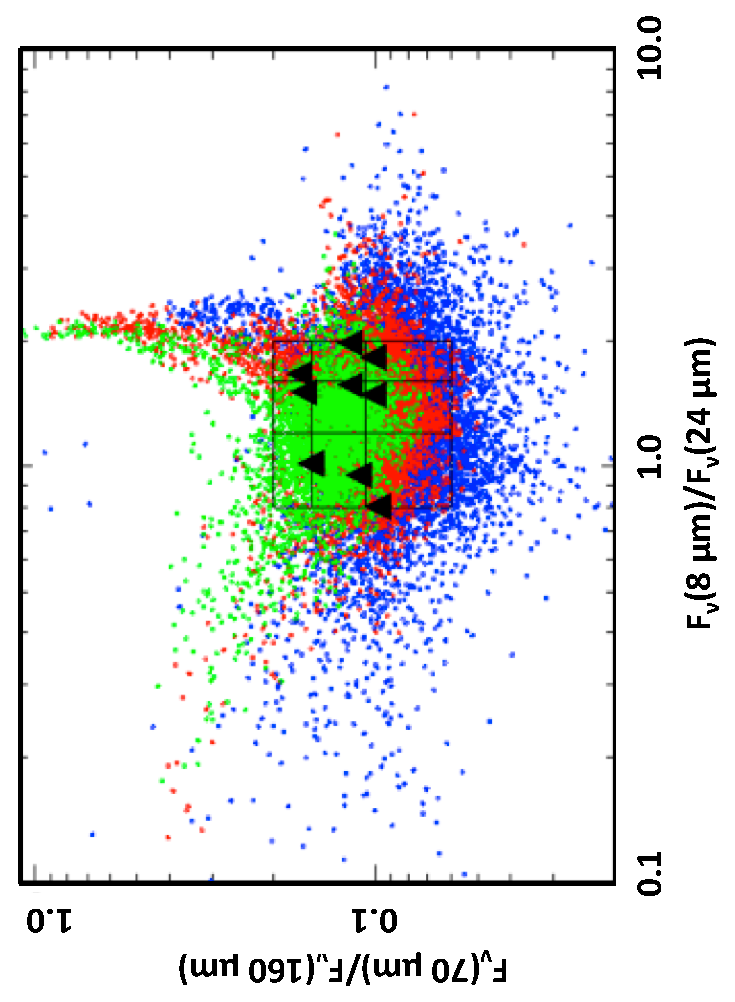
\includegraphics[width = 6.5 cm,angle=270]{fig1.eps}
\caption{$8 - 24/70 - 160$ $\mu$m colour-colour diagram of M31 obtained from IRAC and MIPS imaging. Colour-coding of points represents
24~$\mu$m flux, from faintest (blue) to brightest (red). The plot is divided into 9 regions (black grid), and the observations were made to 
cover those regions subject to a 24~$\mu$m brightness cut. The black triangles indicate colours of the regions we observed.}
\label{colourmaps}
\end{figure}

We obtained mid-infrared spectral maps of 12 regions in M31 using the {\em Spitzer}/IRS instrument \citep{IRS2004} covering wavelengths from 5 to 21 microns. 
A background observation was also made off the galaxy 
along the minor axis for use in background subtraction from the data cubes.
The 12 target regions include the nucleus, the `bulge' and `active' regions previously observed by ISOCAM (the latter is Region 9 in our sample), 
and 9 other regions selected to cover a range of metallicities and dust temperatures.%
\footnote{One additional spectral map in M31 is available in the {\it Spitzer} archive (AOR key 12019200);
unfortunately it does not cover the 5--13~$\mu$m region, which is the major focus of this paper. We therefore elected to not include these observations.} 
These 9 regions were chosen by convolving the IRAC 8~$\mu$m \citep{Barmby2006lr}
and MIPS \citep{gordon06a} maps to the same resolution and constructing an $8 - 24/70 - 160$ $\mu$m colour-colour diagram (Figure~\ref{colourmaps}).
This colour space was used to give a rough definition of the types of spectral energy distribution; the 
dense region in the plot was split into a 3x3 grid and one pixel in each grid region (subject to a 24$\mu$m brightness cut)
was selected for spectroscopy. 
The locations of the observed regions are shown in Figure~\ref{m31}, and 
their coordinates and metallicities are given in Table~\ref{regions}.  
Except for regions 5 and 8, all of our mapped regions contain an  H~{\sc ii} region with
an optical spectroscopic metallicity measurement by \citet{Sanders_2011}; Table ~\ref{regions} gives the measurements from the method 
\citet{Sanders_2011} denote ``N06 N2''  \citep{Nagao2006}. For regions 5 and 8 we estimated metallicities using the M31 radial gradient
that  \citet{Sanders_2011} fit to the H{\sc ii} region ``N06 N2'' measurements: $12+\log{\rm [O/H]} = 9.09 - 0.00195 R{\rm gc}$.

\begin{table*}
 \centering
 \begin{minipage}{90mm}
\caption{Spitzer/IRS Target Locations in M31
\label{regions}}
\begin{tabular}{lccrl}
\hline Name & R.A. (J2000) & Decl. (J2000) & ${R_{\rm gc}}^b$ & $12+\log({\rm O/H})^c$
\\
 \hline
Nucleus$^a$ & $00^{\rmn{h}}42^{\rmn{m}}44\fs31$ & $41\degr16\arcmin09\farcs4$  & 0.0 & \\
Bulge$^a$   & $00^{\rmn{h}}42^{\rmn{m}}35\fs00$ & $41\degr21\arcmin01\farcs0$  & 4.7 &$8.90\pm0.03$\\
Region 1    & $00^{\rmn{h}}41^{\rmn{m}}30\fs41$ & $40\degr43\arcmin07\farcs8$  & 12.4 &$9.20\pm0.20$\\
Region 2    & $00^{\rmn{h}}45^{\rmn{m}}22\fs85$ & $41\degr38\arcmin53\farcs1$  & 13.0 &$9.07\pm0.02$\\
Region 3    & $00^{\rmn{h}}40^{\rmn{m}}37\fs37$ & $41\degr01\arcmin29\farcs4$  & 12.1 &$8.85\pm0.01$\\
Region 4    & $00^{\rmn{h}}41^{\rmn{m}}17\fs86$ & $41\degr07\arcmin09\farcs8$  & 8.7 &$8.89\pm0.06$\\
Region 5    & $00^{\rmn{h}}43^{\rmn{m}}39\fs57$ & $41\degr19\arcmin03\farcs1$  & 7.0 &$8.93\pm0.08$\\
Region 6    & $00^{\rmn{h}}43^{\rmn{m}}35\fs72$ & $41\degr23\arcmin15\farcs0$  & 4.3 &$8.73\pm0.08$\\
Region 7    & $00^{\rmn{h}}40^{\rmn{m}}53\fs98$ & $40\degr58\arcmin58\farcs9$  & 8.7 &$8.40\pm0.08$\\
Region 8    & $00^{\rmn{h}}42^{\rmn{m}}21\fs60$ & $41\degr07\arcmin17\farcs4$  & 3.1 &$8.94\pm0.08$\\
Region 9$^a$& $00^{\rmn{h}}41^{\rmn{m}}00\fs00$ & $40\degr36\arcmin20\farcs3$  & 13.5 &$8.86\pm0.02$\\
NGC~206     & $00^{\rmn{h}}40^{\rmn{m}}20\fs20$ & $40\degr44\arcmin54\farcs0$  & 9.8 & \\
Background  & $00^{\rmn{h}}44^{\rmn{m}}41\fs80 $ & $40\degr58\arcmin56\farcs0$  & 29.5 & \\
\hline
\end{tabular}
{$^a$Regions with ISOCAM data.\\
$^b$De-projected galactocentric distance in kpc.\\ 
$^c$Metallicities from \citet{Sanders_2011}, except for Regions 5 and 8 where metallicities are estimated from the radial metallicity profile.
}
\end{minipage}
\end{table*}

\begin{figure*}
\centering
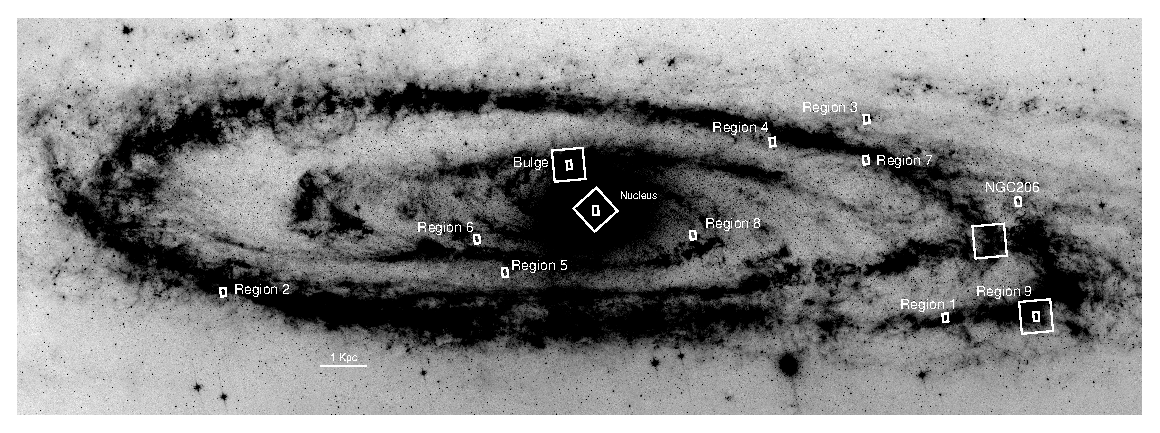
\includegraphics[scale=0.9]{./fig2.eps}
\caption{An 8 micron negative IRAC image of M31 \citep{Barmby2006lr}. Small white rectangles ($30\arcsec\times50\arcsec$) show the regions that we observed, and larger squares ($192\arcsec\times192\arcsec$) show the regions observed by  \citet{1998Cesarsky}.
\label{m31}
}
\end{figure*}


For our observations we used the IRS Short-Low (SL) and Long-Low (LL) modules, which cover wavelengths from 5 to 21 microns. 
The Low modules have resolving power in the range 60--130. Each low-resolution module is divided into two sub-slits 
which provide spectroscopy in either first or second order. They are denoted as SL1 (7.5--14.5~$\mu$m), SL2 (5.2--7.6~$\mu$m),
LL1 (20.5--38.5~$\mu$m, not used in these observations), and LL2 (14.5--20.75~$\mu$m).
All M31 regions were observed in September 2007 as part of G. G. Fazio's Guaranteed Time (program ID 40032). 
The map size was based on the size 
of the IRS slits (SL: $3.6\arcsec \times 57\arcsec$, LL: $10.5\arcsec \times 168\arcsec$). Each region was covered by 18 overlapping observations 
of the SL slit and 11 overlapping observations of the LL slit making the map size $32\arcsec \times 57\arcsec$ for SL and $58\arcsec \times 168\arcsec$ for LL. 
Figure~\ref{slits} shows an example of the slit arrangement. For the brighter regions (nucleus, bulge), ramp times of 14 s (SL) and 30 s (LL) were used, 
while for the fainter regions, ramp times of 60 and 120 s were used respectively. Background observations were taken with each module (2 per ramp time). 
Because all of the targets are in the same part of the sky, a common background observation was used for multiple targets to subtract the background emission. 

\begin{figure}
\centering
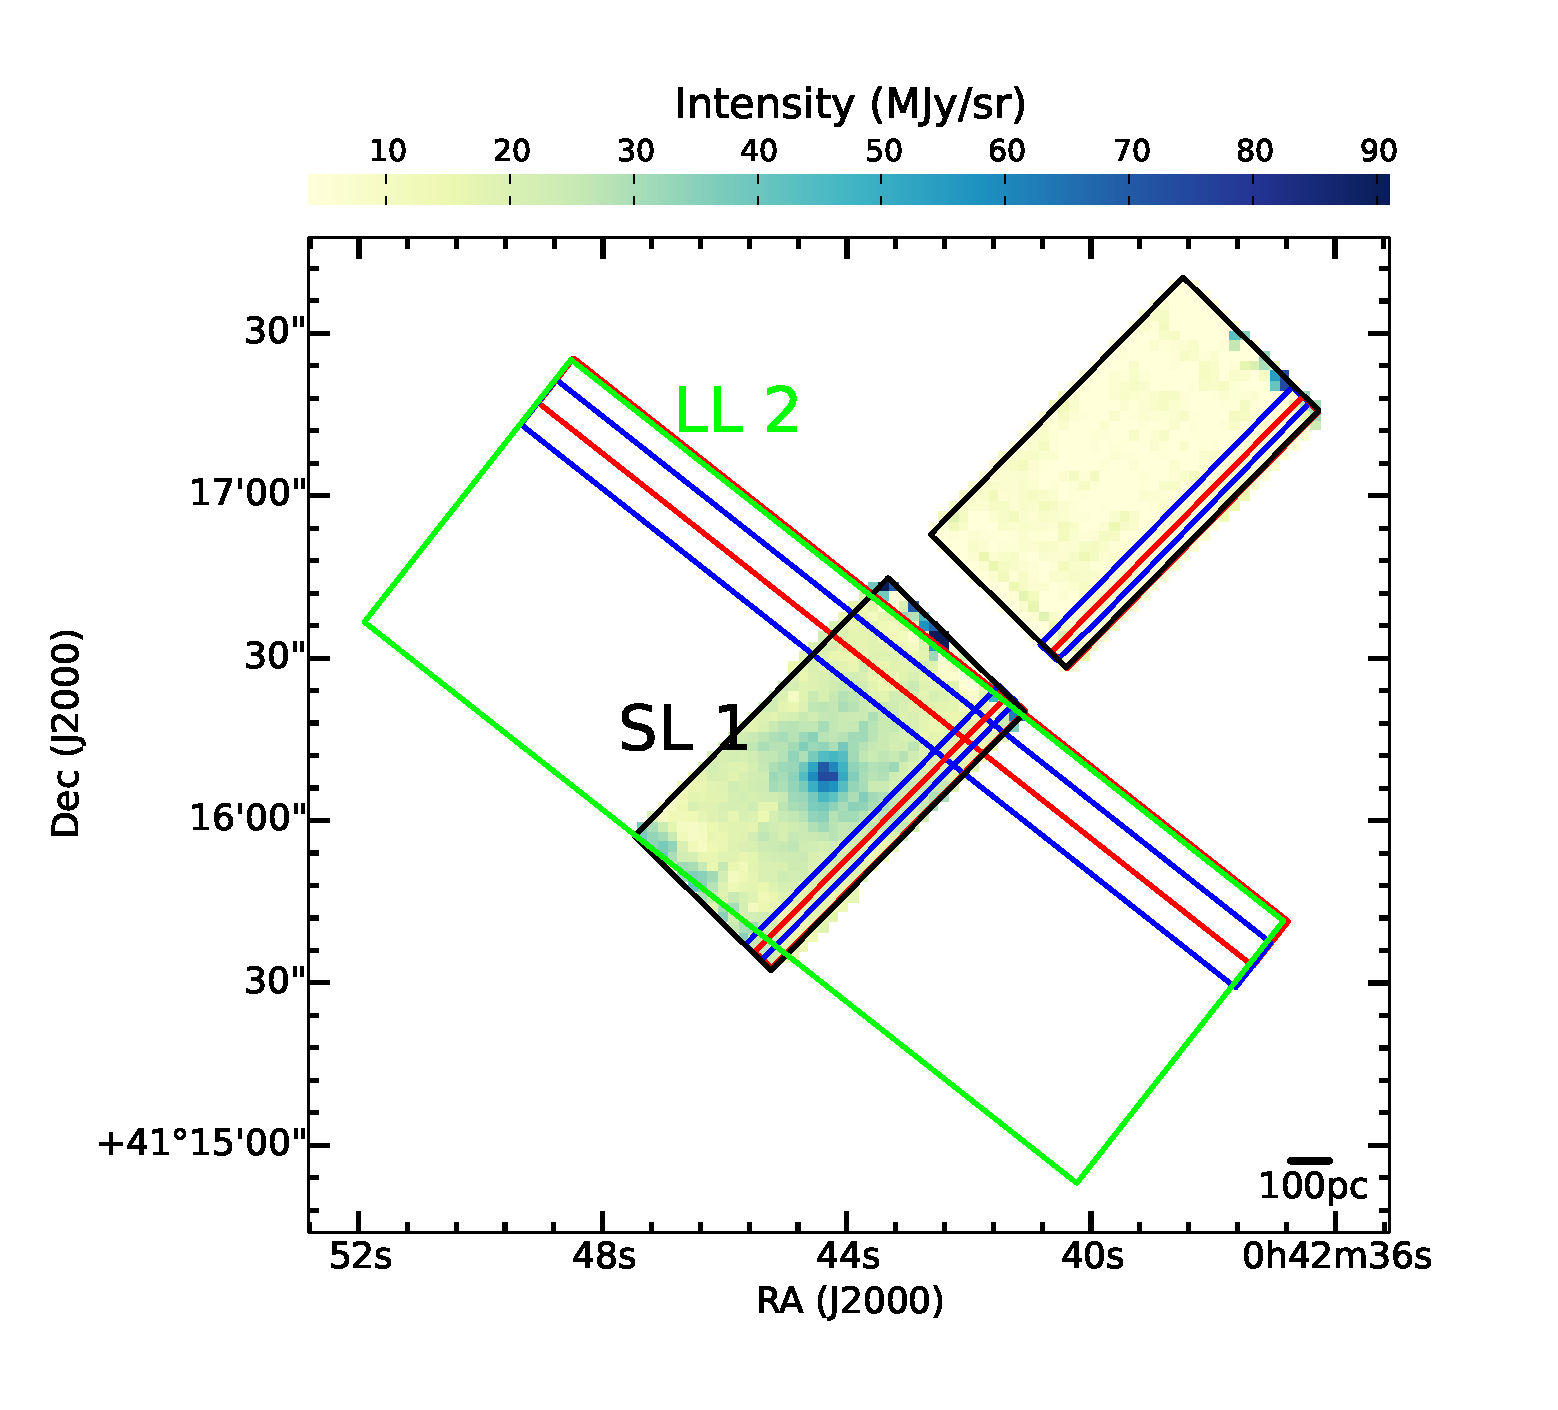
\includegraphics[scale=0.3]{./fig3.eps}
\caption{The 7.6~$\mu$m plane constructed from the SL1 data cube of the nucleus, showing the arrangement of slits used to cover the region. 
Black boxes outline the footprint of the SL1 maps (the off-center SL1 map is from observations made
when SL2 was centred) and the green box outlines the LL2 map. 
Blue and red slits show how  each map was covered using overlapping slit positions.
\label{slits}
}
\end{figure}

\subsection{IRS Data Reduction}
\label{sect:irs_data}

The data were reduced through the SSC pipeline (ver. S17.2.0), and the maps were assembled using the CUBISM program \citep{Smith:2007fk}. 
Bad pixel removal was also done using CUBISM, and the background observations were used to subtract the background emission from these cubes 
following the method outlined by \citet{Gordon:2008lr}. Spectra were extracted using a $30\arcsec\times50\arcsec$   rectangular aperture,
which corresponds to $114\times190$~pc at the distance of M31.
The aperture size was selected to cover the overlapping area of the SL and LL modes; all the IRS maps cover more area than  considered here.
In order to study the spatial variation of the emission near the nucleus, we also extracted spectra from two smaller regions
within that map; these will be further discussed in Section~\ref{sect:nucleus}.
The spectrum of NGC 206 is very noisy and was removed from our analysis. 

% REF:
%Section 2.2:
%Why did you not include the bonus order (SL3) data to help in the overlap regions of the SL matching?
%
%There is a synthetic IRAC 4 tool inside CUBISM which takes the spectral cube and produces a map as it would be observed through the IRAC 4 filter. Comparing this map with the map from Barmby et al 2006 and deriving a correction factor seems to be more straight-forward than the method you describe.
%
%I did not understand ***why*** the SL and LL orders do not match naturally and instead have a systematic offset. Also the calculated offset (table 2) is positively correlated with the IRAC 4 photometry, why?
%
%The statement about the non-zero intercept and thus opting to apply an offset correcting is unconvincing given that you find an offset compatible with 0 (-0.05 +- 0.06) and a slope which is significantly different than unity.


There is wavelength overlap between the SL1 and SL2 spectra and also between the SL1 and LL2 spectra.
To generate a single spectrum for each M31 region it is necessary to combine the spectra and
account for photometric offsets between them. Such offsets are commonly seen in IRS spectra extracted
from extended regions, since the slit loss is not well-characterized (**Els please check this sentence**).
The SL1 and SL2 flux densities were
generally quite well-matched over the wavelength overlap region ($7.5 < \lambda< 7.6\mu$m)
and those two orders were combined by averaging fluxes over the  overlap region.
In cases with offsets between SL1 and SL2, we found that SL2 and the `bonus order' SL3 were well-matched.
We  combined the  SL1 and SL3 
spectra by computing the average flux densities over the  overlap region and
adding a constant  to the SL1 spectra so that they matched the SL3 average. The SL1 and SL2 orders
were then combined as described above.
After this procedure there was still a noticeable mis-match between the SL and LL spectra. We addressed this
by scaling the SL spectra to match IRAC 8~$\mu$m fluxes as follows. IRAC fluxes were measured
on the 8~$\mu$m image \citep{Barmby2006lr} in the same apertures used to extract the IRS spectra.
An extended source  aperture correction of 0.824 was applied to the IRAC fluxes; this value was computed 
using the formula in the IRAC Data Handbook \citep{} with
the radius of a circular aperture having the same area as the extraction aperture.
The {\em Spitzer} synthetic photometry software \citep{SpitzerDAC} 
was then used to quantify the colour correction for each spectrum, i.e. the
multiplicative factor $K$ between the IRAC photometry over its broad bandpass and the IRS flux
density at the centre of the bandpass.  For each spectrum we computed the additive
offset between the color-corrected IRS flux density and the IRAC aperture-corrected flux density,
and used this to correct the SL spectra; this method was also used by \citet{Sandstrom12}.
Although a multiplicative offset could also have been used to match the IRS photometry to IRAC,
the resulting change in spectral slope increased the size of the SL/LL offset.
The SL spectra corrected with additive offsets were closely-matched to the LL spectra, and the final combination
of SL and LL was done using the average-and-offset procedure described above for SL1 and SL3.



\subsection{ISOCAM Data Reduction}
\label{sect:iso_data}

To compare our results with those of  \citet{1998Cesarsky}, we retrieved the highly processed ISOCAM data provided by \citet{Boulanger_F_2005}  
for the nucleus, bulge, and region 9. 
The ISOCAM data were obtained with the circular variable filters (CVFs) over a $3\arcmin \times 3\arcmin$ field of view at a scale of 6\arcsec\ per pixel. 
The wavelength range covered was 5.15--16.5~$\mu$m at a resolution of $\lambda/\Delta \lambda \approx 45$; the ISOCAM instrument is described by \citet{cesarsky1996}.
An example image of the ISOCAM data is shown in Figure~\ref{isonuc}.  For the three regions, we extracted spectra using the same 
$30\arcsec\times50\arcsec$ aperture as for the IRS data. 

\begin{figure}
\centering
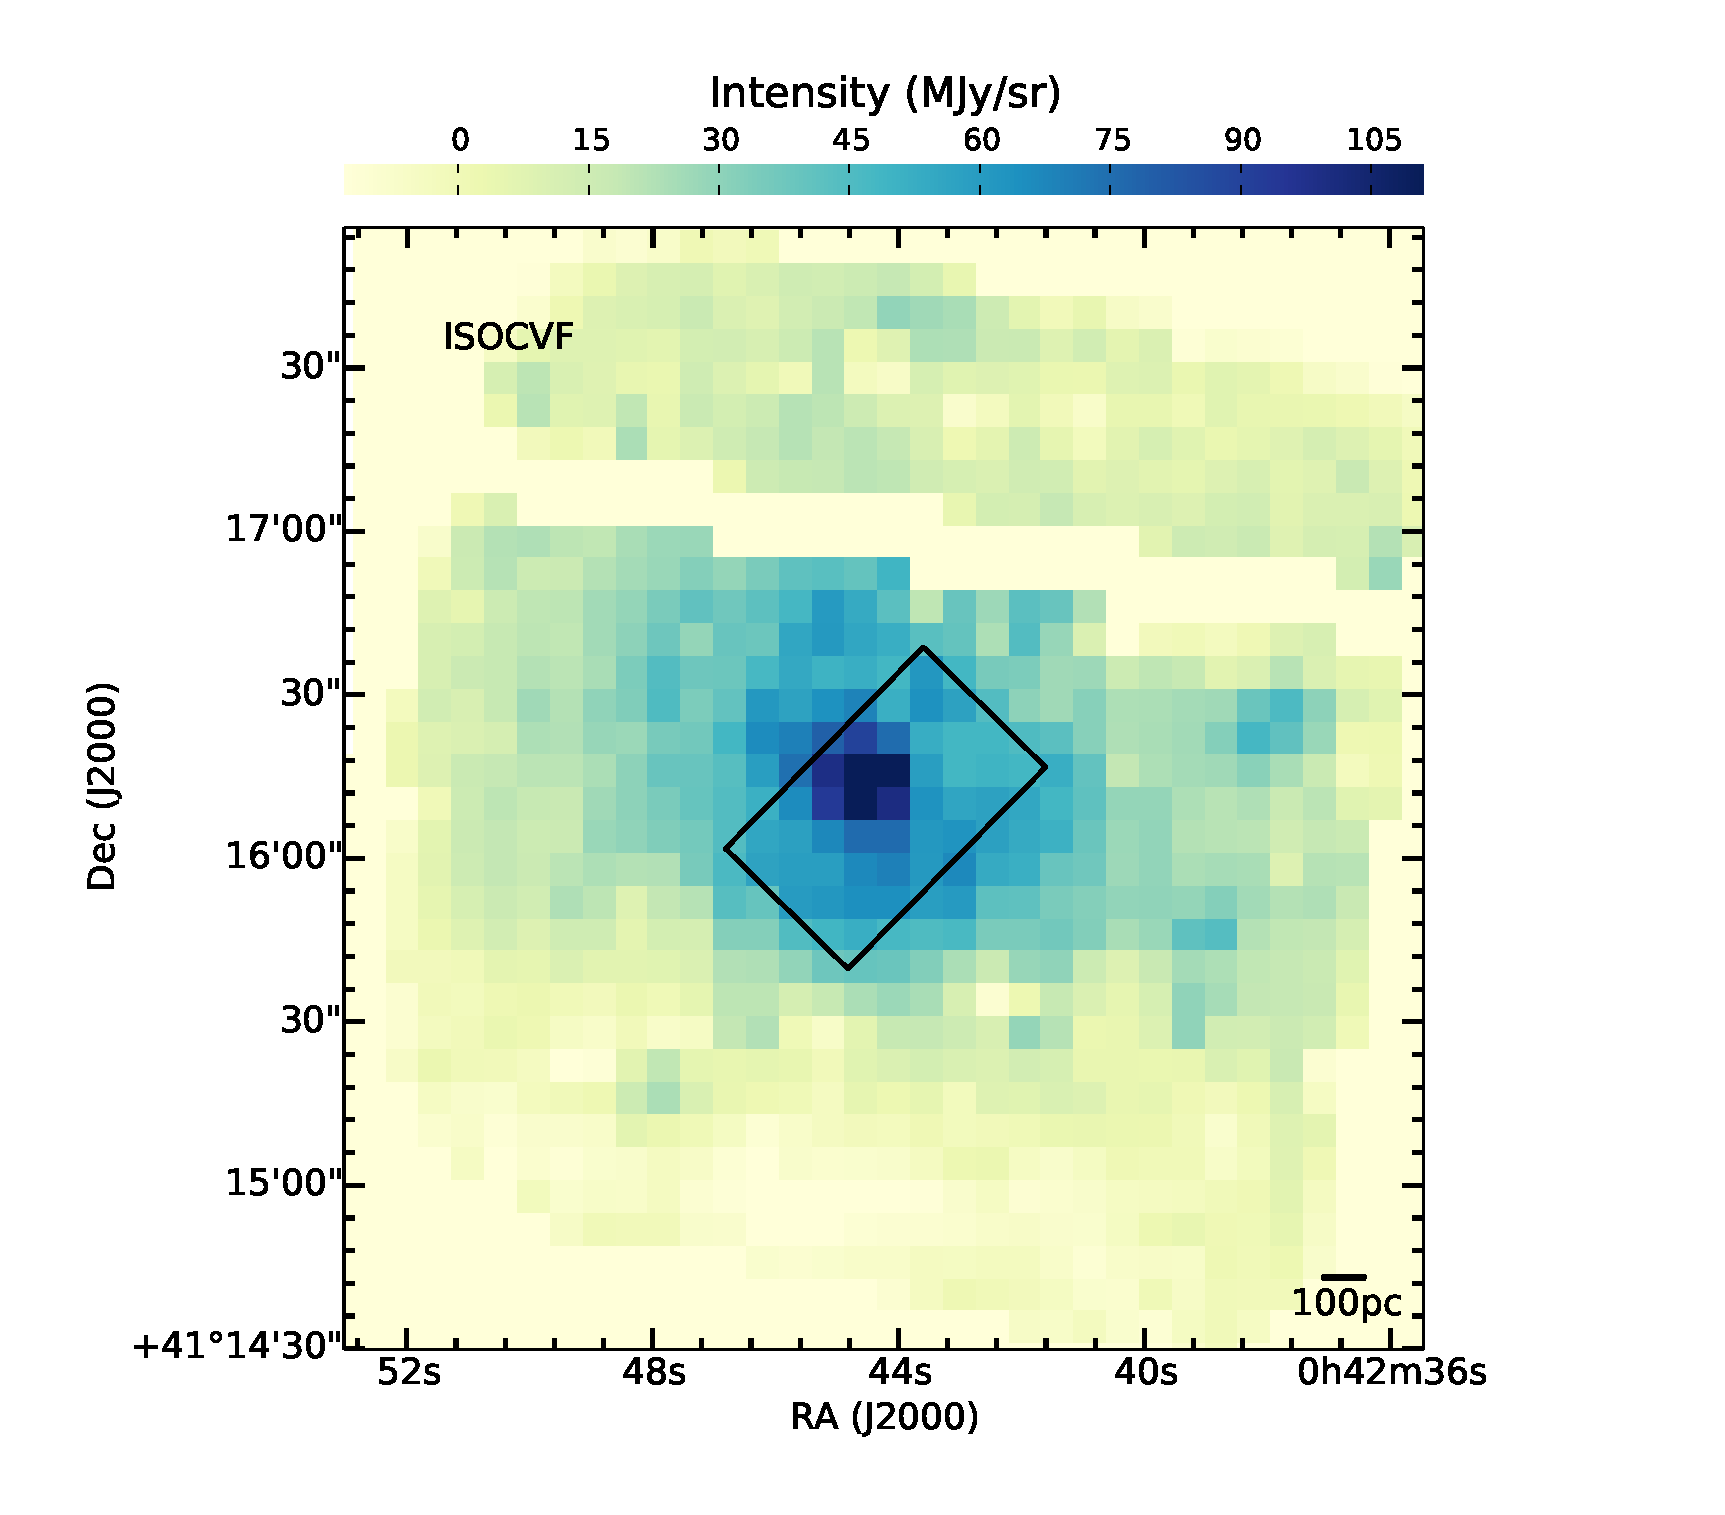
\includegraphics[width = 8cm]{./fig4.eps}
\caption{11.3~$\mu$m negative image (dark colours indicate higher flux) of the ISOCAM data cube from the nucleus of M31. 
The black box shows the size of the aperture ($30\arcsec\times50\arcsec$) used to extract spectra.}
\label{isonuc}
\end{figure}





